\documentclass[border=3pt,tikz]{standalone}
\usepackage[utf8]{vietnam}
\usetikzlibrary{calc,angles,intersections,shapes.geometric,arrows,decorations.markings,arrows.meta,patterns.meta,patterns}
\usepackage{tikz-3dplot,pgfplots}
\pgfplotsset{compat=1.15}
\usepgfplotslibrary{polar}
\usepackage{amsmath}
\begin{document}
	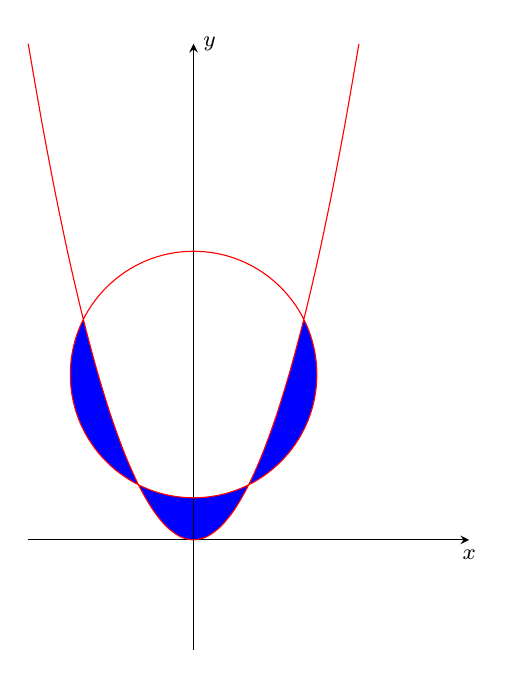
\begin{tikzpicture}[scale=0.7, font=\footnotesize,>=stealth]
		\def\f(#1,#2){plot [smooth,domain=#1:#2](\x,{(\x)^2})}
		\def\c{(0,3) circle ({sqrt(5)})}
		\begin{scope}
			\clip \c (-3,0) rectangle (3,9);
			\fill[blue] \f(-2,2);
		\end{scope}
		\begin{scope}
			\clip \f(-3,3) |-(-3,0)--cycle;
			\fill[blue]\c;
		\end{scope}
		\draw[->] (-3,0)--(5,0) node [below] {$x$};
		\draw[->] (0,-2)--(0,9) node [right] {$y$};
		\draw[red] \f(-3,3) \c;
	\end{tikzpicture}
\end{document}